\section{Gleisplan}
\label{sec:map}

Dieses Kapitel stellt den aktuellen Gleisplan vor, geht aber auch auf seine historische Entwicklung ein.
Der Fokus liegt darauf, diese Entwicklung anhand der Entscheidungshintergr\"unde zu dokumentieren.
Es wird deshalb auch auf verfolgte Betriebsszenarien sowie den zugeh\"origen Dioramabau eingegangen.
Diese beiden Aspekte werden aber nachfolgend noch in unabh\"angigen Kapitel vertieft.

Da das Thema von Granitz in einer relativ flachen, Brandenburger Landschaft versiedelt ist, gibt es wenige echte Tunnels.
Zur Planung des Gleisgrundrisses wurde daher weitestgehend die Freeware \textit{Trackplanner} \cite{W\"ac07} verwendet.
Bei einigen der nachfolgenden Abbildungen handelt es sich um exportierte, i.d.R. nachbearbeitete Bilder aus der Software.
Der digitale Appendix enth\"alt zudem die Gleisplandateien im Trackplanner-typischen Format \textit{.glp}.

Nachfolgend wird zuerst die Historie des Gleisplans abgehandelt (Sec.~\ref{sec:map_basicHistory}-\ref{sec:map_history}).
Die jeweils aktuelle Ausbaustufe und der Gleisplan f\"ur die projektierte Endausbaustufe folgen in den anderen Unterkapiteln (Sec.~\ref{sec:map_date}-\ref{sec:map_final_projected}).

\subsection{Grunds\"atzliche Planungsgeschichte}
\label{sec:map_basicHistory}

Der Plan sah von Anfang an eine zweigleisige Hauptstrecke mit mindestens einer eingleisigen Nebenstrecken vor.
Es sollte dabei ein gutes Gleichgewicht zwischen Betriebsm\"oglichkeiten (Spiel) und szenerischer Gestaltung gefunden werden.
Im Fokus stand zun\"achst eine einfache Realisierung unter deutlicher Inkaufnahme einer Verminderung des realen Betriebsgeschehens.
Das typische Oval war dementsprechend die Grundidee.
Dieser Startschuss f\"ur Granitz kann auf \hl{ca. Weihnachten 2015} datiert werden.

Anf\"anglich war auch noch nicht klar, wann bzw. ob \"uberhaupt eine Umsetzung der Anlage ausgef\"uhrt werden k\"onnte.
Der Hauptgrund war wie so \"ublich der Platzmangel in der eigenen Wohnung, weniger der Zeitaspekt.
Im Gegenteil war letzterer absolut nachrangig, da ohnehin ein neues Hobby gesucht wurde, in dem Computer mit Hardwaresteuerung und einem vorzeigbaren Output w\"unschenswerte Bestandteile waren.

Die Arbeiten am Gleisplan wurden jeweils um Weihnachten 2018 und 2019 wiederaufgenommen.
Im Januar 2020 fiel dann auch der Entschluss, das Vorhaben tats\"achlich zu realisieren.
Durch den nach wie vor bestehenden Platzmangel wurden zun\"achst Wege gesucht, die Anlage zu segmentieren.
Ma{\ss}geblich waren in diesem Zusammenhang auch Inspirationen aus Beitr\"agen, die auf der Seite \textit{moba-trickkiste.de} zusammengestellt sind.
Insbesondere ist hier der Beitrag \textit{Vom Kreisverkehr zum Betriebserlebnis} \cite{Gee17} zu nennen.
Dadurch wurde aus dem Konzept eine segmentierten Zentralplatte eine L-Form gemacht, die zu einem sp\"ateren Zeitpunkt in eine U-Form \"uberf\"uhrbar w\"are.
Die wichtigsten verarbeiteten Aspekte waren hierbei:
\begin{itemize}
	\item Raumausnutzung und An-der-Wand-F\"uhrung, was insbesondere in Plattenschenkeln von maximal 100cm Tiefe, bevorzugt weniger resultierte
	\item Ann\"aherung des Gleisplans an das Punkt-zu-Punkt Konzept
\end{itemize}
Ein weiterer Aspekt, der f\"ur Granitz aber nicht wirklich umgesetzt wurde, ist die Erkenntnis, dass eingleisige Nebenstrecken offenbar wirklich einfacher und realistischer zu bauen sind.
Sehr weit in die Zukunft schauend, w\"urden Erweiterungen oder Neubauten daher sicherlich vom zweigleisigen Hauptstreckenkonzept Abstand nehmen.

Wie man sieht, kann das Lesen aus den Erfahrungssch\"atzen anderer eine wirklich gro{\ss}e Hilfe ist.
Mir pers\"onlich dient das zum Brinstorming und nat\"urlich auch zum aus den Fehlern anderer lernen.
Gleichwohl kann man hier und dort immer stur bleiben und den eigenen Vorstellungen folgen - das schlie{\ss}t sich nicht aus und der Spa{\ss} am T\"ufteln muss ja erhalten bleiben.

Was in Hinblick auf \cite{Gee17} noch peripher erw\"ahnt sein soll - kurz losgel\"ost von der Gleisplanthematik:
Das Erz\"ahlen der fiktiven Geschichte hinter der Anlage ist denke ich sehr wichtig, um sich nicht nur selbst den Fahrplan zu legen, sondern die Anlage auch f\"ur Dritte verst\"andlich zu machen.
Aus diesem Grund erstelle ich auch die Dokumentation und es war mir ein Anliegen, die Stadt Granitz in Sec.~\ref{sec:storyOfGranitz} vorzustellen.
Das erkl\"art dann auch schon in weiten Teilen den Hintergrund zum Gleisplan, Betrieb, Szenerie etc.


\subsection{Entwicklungsstadien}
\label{sec:map_history}

\subsubsection{Das Oval}
\label{sec:map_development_state1}

Der etwaige Erstentwurf aus dem Jahr \hl{2015} sowie die Wiederbelebung nach Weihnachten 2018 sind in Fig.~\ref{img:state0-1_granitz_modules_details} dargestellt.
Meiner Erinnerung nach sind die einzigen Unterschiede das Fehlen der kompletten Schattenbahnhofsebene sowie des linksoben angeflanschten Nebenszenarios (Minibahnhof) - dies war im Erstentwurf nicht enthalten.
Stattdessen sollte linksoben eine \"Uberf\"uhrungsm\"oglichkeit zur Anlage meines Vaters freigehalten werden.
Die \"Uberf\"uhrung rechtsoben war jederzeit untergeordnet, da hier keine konkreten Pl\"ane vorlagen.
Eine Vereinigung mit einer Anlage meines Bruders war noch am ehesten in meiner Vorstellung.

Die Abbildung enth\"alt bereits eine Segmentierung, um die gut $2~m \cdot 3~m$ gro{\ss}e Anlage irgendwo verstauen zu k\"onnen.
Der mittlere Segmentriegel wurde in die beiden \"au{\ss}eren Bahntrassensegmente und die zentralen Dioramasegmente unterteilt, um letztere v\"ollig unabh\"angig entwickeln und bei Bedarf sogar ersetzen zu k\"onnen.

Das angeflanschte Segment mit dem Minibahnhof wurde als kleines, aber feines Diorama Highlight geplant.
Hier sollte ein sehr, sehr niedrig frequentierter Haltepunkt eingef\"ugt werden, der bei Ausfl\"uglern sehr beliebt ist.
Der Halt sollte auf einer Erhebung sein mit Ausblick auf den n\"ordlichen, etwa $10~cm$ tiefer gelegenen Anlagenriegel.
Noch vor der Kurve der Hauptstrecke sollte eine beschauliche Wiese mit einem kleinen Teich angelegt werden.
Die Kurve der Hauptstrecke wurde relativ bald unter das Terrain verlegt, um die Landschaft hier noch etwas weiter zu ziehen.
\begin{itemize}
	\item Das Diorama ist auch noch aktuell in Planung und wird als Bahnhof \textbf{Sch\"onblick} gelistet.
\end{itemize}

Der Regionalzug- und Bummelzughalt, oben zentral eingezeichnet, sollte als Endpunkt der hier sehr kurzen Nebenstrecke und optionaler Regionalzuhalt dienen.
Hier sollte ein durch einen Wald abgetrennter, ggf. eingemeindeter Ortsteil von Granitz angedeutet sein, urspr\"unglich als \textbf{Granitzer Heide} gelistet.
Westlich von der Bahnhofsausfahrt ergibt sich neben der Gleisf\"uhrung nach Sch\"onblick au{\ss}erdem eine Abfahrt in die Schattenbahnhofsebene, potenziell f\"ur den G\"utervekehr.
\begin{itemize}
	\item Der Regionalzughalt ist in der aktuellen Planung als Bahnhof \textbf{Granitz-Walddorf} umgewidmet.
	\item Dioramatechnisch sehen alle fortgeschrittenen Planungen eine Trennung dieses Bahnhofs von der benachbarten \textbf{Gleisaufgabelung} vor.
\end{itemize}

Die zentralen Panoramasegmente sowie das Segment der Stadt Granitz selbst sind aus Fig.~\ref{img:state0-1_granitz_modules_details} heraus selbsterkl\"arend.
Der Schattenbahnhof hat allein die Funktion von Abstellgleisen und einer gro{\ss}en Wendeschleife, die zwischen Nordwest und S\"udost befahren werden kann.
Allein ein Merkmal soll hier explizit aufgef\"uhrt werden, das f\"ur alle Entwurfsphasen mandatorisch war und ist:
\begin{itemize}
	\item Bahnsteige m\"ussen eine Kapazit\"at von mindestens f\"unf (Fernverkehr) bzw. vier  (Regionalverkehr) Personenwagen aufweisen.
	Dies gibt somit die Bahnsteigl\"angen in Granitz sowie am Regionalhalt vor.
	\item Eine Kapazit\"at von sechs Personenwagen in Granitz ist dar\"uber hinaus ausdr\"ucklich angestrebt.
\end{itemize}

Modelleisenbahnanlagenbau kann viel Zeit in Anspruch nehmen.
F\"ur mich war und ist es wichtig, bald schon mal einen Zug fahren lassen zu k\"onnen.
Zusammen mit den bereits angedeuteten Problemen bzgl. Platzmangels in der Wohnung wurde schon sehr fr\"uh die Modularisierung in Segmente auf den Plan gesetzt.
Insbesondere 2018 erschien es als absolut unrealistisch, eine Plattentiefe von $2m$ in der Wohnung zu realisieren.
Als Kombil\"osung beide Aspekte betreffend wurde die komplette Entnahme des mittleren Segmentriegels als Option geplant, s. Fig.~\ref{img:state0-1_granitz_modules_compressed}.

Dies erfordert f\"ur eine Anpassung der (urspr\"unglichen) finalen Anlage gem\"a{\ss} Fig.~\ref{img:state0-1_granitz_modules_details} wenig \"Anderungen an der Gleisf\"uhrung:
\begin{enumerate}
	\item Die Nebenstrecke braucht eine alternative, flachere Zuf\"uhrung zum Regionalhalt.
	Dies kann auch bei einem m\"oglichen Hin- und Herwechseln zwischen der komprimierten und Vollvariante bestehen bleiben, indem \"uber eine zus\"atzliche, am Westausgang vom Bummelzughalt einzubauende Weiche (hier nicht abgebildet) jeweils das nicht genutzt Gleis als Totgleis definiert wird.
	\item Der westliche Schleifenschluss in der Schattenbahnhofsebene erfordert eine geringf\"ugige Anpassung.
\end{enumerate}
Es sei darauf verwiesen, dass der mittlere Segmentriegel mit eine Tiefe von $55.5~cm$ bemessen wurde, dementsprechend auf Standardl\"angen vom verwendeten Gleismaterial ausgelegt wurde.

Als zus\"atzliche Information enth\"alt Fig.~\ref{img:state0-1_granitz_modules_compressed} verschiedene Baulose f\"ur den Bastler.
Diese waren sowohl in zeitlich und gestalterisch sinnvolle Abschnitte unterteilt als auch in Budgetierungsabschnitte, um den geringen Gleisbestand aus der Kinderanlage haushaltspolitisch vertr\"aglich zu erweitern.

\begin{figure}[h]
\centering
	\begin{subfigure}[b]{1.0\textwidth}
    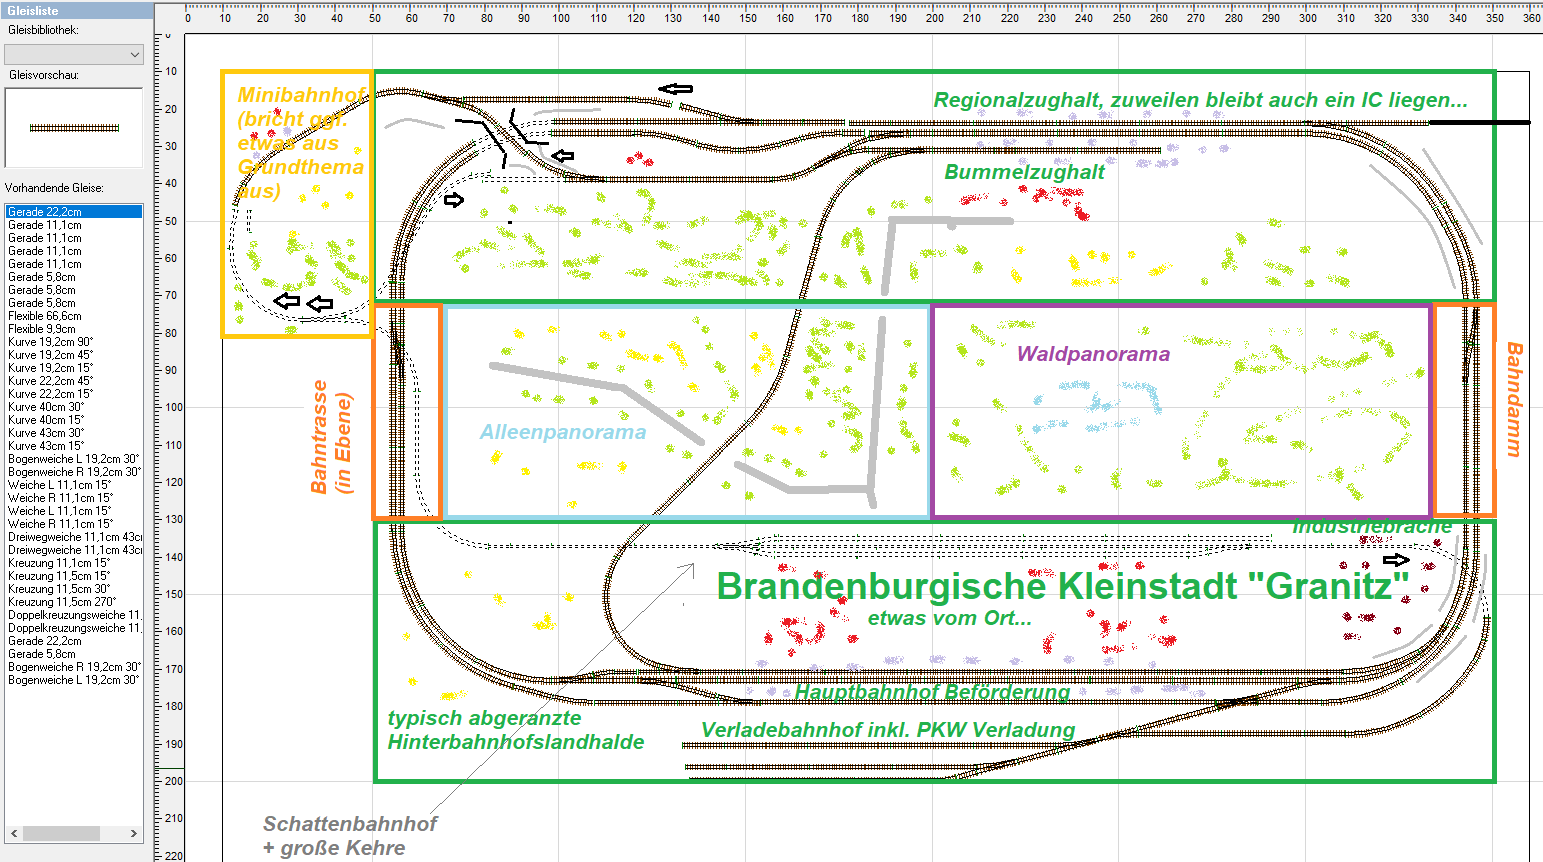
\includegraphics[width=1.0\textwidth]{img/map_evolution/state0-1_granitz_modules_details.png}
   \caption{Urspr\"ungliche Planung f\"ur Vollausbau}
    \label{img:state0-1_granitz_modules_details}
    \end{subfigure}
	\begin{subfigure}[b]{1.0\textwidth}
    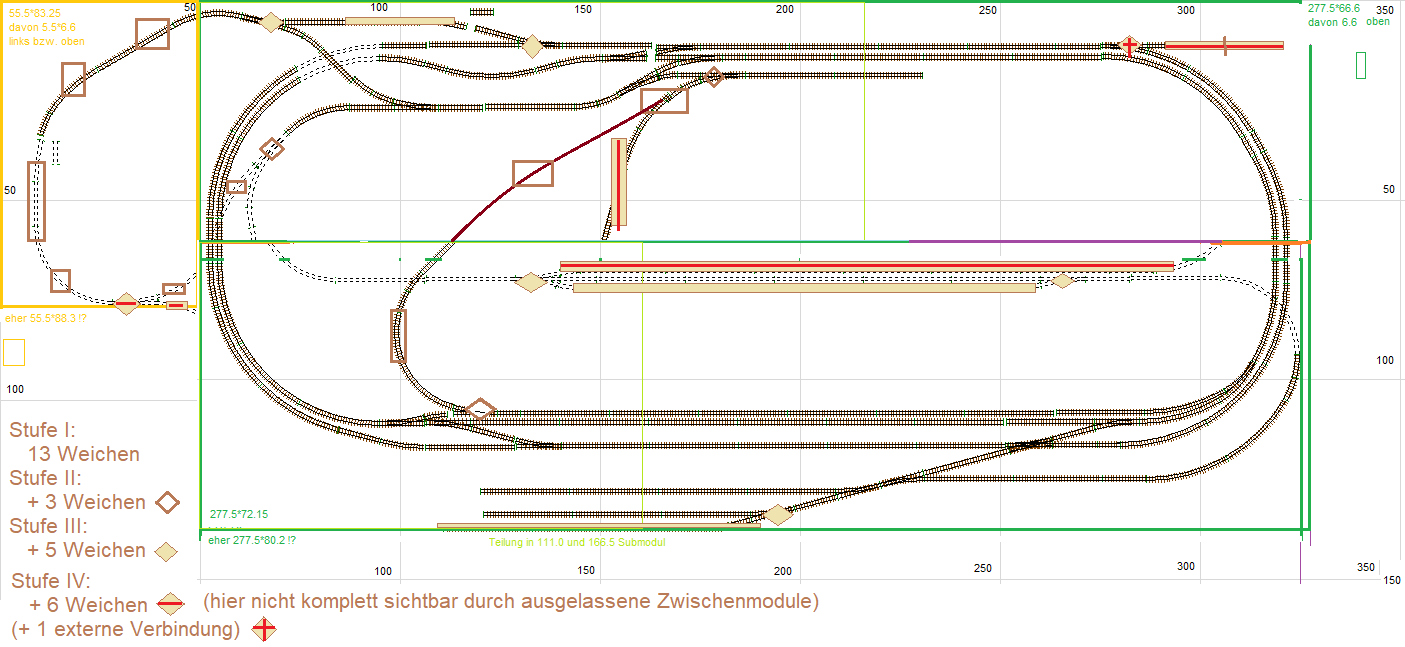
\includegraphics[width=1.0\textwidth]{img/map_evolution/state0-1_granitz_modules_compressed.png}
   \caption{Komprimierte Anlage f\"ur fr\"uhe Ausbaustadien}
    \label{img:state0-1_granitz_modules_compressed}
    \end{subfigure}
	\caption{Erste Entwurfsserie, ausgef\"uhrt als segmentierte Rechteckanlage}
	\label{img:state0-1_granitz}
\end{figure}

Letztendlich entsprechen diese Erstentw\"urfe dem klassischen Oval mit etwas Nebenstreckenfirlefans.
Das war dem Autor fr\"uh bewusst aber auch okay so.
Es ging darum, mal einen Zug fahren zu lassen, etwas \"uber die Nebenstrecken und mit dem Schattenbahnhof zu variieren und sich vor allem an den beiden Panoramaplatten gestalterisch auszutoben.
Siehe hierzu auch die in der Einleitung beschriebene Geisterung f\"ur Brandenburg und das ganze drum herum.
Die Fahrstrecke zwischen Granitz und dem Regionalhalt war mit ca. $3m$ (\"uber Granitz-West) bzw. ca. $2m$ (\"uber Granitz-Ost) auch annehmbar.


\subsubsection{Wage Ann\"aherung an den Hundeknochen \"uber die Abgeknickte Acht}
\label{sec:map_development_state2}

Der Entschluss einer tats\"achlichen Umsetzung der Anlage konnte aus Platzgr\"unden nur durch eine konstruktive, ggf. radikale Abwandlung erfolgen.
Wie bereits erw\"ahnt, hat mir der Input von \cite{Gee17} ungemein dabei geholfen, den Prozess geistig in Gang zu setzen.

Der offensichtlichste Nachteil des Ovalkonzepts blieb die Klobigkeit.
Eine Tiefe von $2~m$ verhindert zwangsl\"aufig die Aufstellung an der Wand, da es fr\"uher oder sp\"ater zu Entgleisungen etc. kommen muss.
Der zus\"atzlich einzuplanende und vor allem freizuhaltende Durchgangsbereich macht ein Raumkonzept schnell zunichte.
In dem Raum, wo Granitz nun aufgebaut wird, stand vormals ein Kickertisch, der schon viel Platz in Beschlag genommen hat, aber eine Korpustiefe von $75~cm$.

Gleichzeitig ist das pure Oval nat\"urlich auch nicht besonders attraktiv.
Eine Auffaltung des Anlagenkonzepts bietet demgegen\"uber neue Optionen unter der Voraussetzung, selbst unter der Anname, dass die Grundfl\"ache der Anlage konstant bleibt:
\begin{itemize}
	\item Die Fahrstrecke wird automatisch verl\"angert.
	Ein Beispiel hierf\"ur sei das Umarrangieren des Ovals zu einer Banane oder Umfalten zu einer abgeknickten Acht:
	\begin{itemize}
		\item Die weniger tiefen Segmente in L-Anordnung erfordern mehr Strecke, da der Weg sinnbildlich zur\"uckgefahren werden muss.
		\item Die l\"angere Strecke resultiert zugleich in einer l\"angeren und somit etwas realistischeren Fahrzeit zwischen den Bahnh\"ofen.
		\item Eine Option ist, die zus\"atzliche Strecke ebenfalls in die Ebene 0 zu legen.
		F\"ur ein Brandenburger Thema geht dabei viel Platz f\"ur das Diorama verloren (gro{\ss}er Nachteil).
		F\"ur ein Thema im Mittelgebirge oder Voralpenland ist dies \"uber Tunnels auffangbar.
		\item Die zweite Option ist, die zus\"atzliche Strecke in die Schattenbahnhofsebene zu verlegen.
		Das wurde hier gemacht.
		Ein Nachteil ist, dass dadurch auch potenzielle Panoramastrecke verlorengeht bzw. der Zug die meiste Zeit unsichtbar ist.
		Dieser Nachteil besteht beim normalen Tunnel aber ebenfalls und ist allgemeinhin aus Autorensicht ein absolut gangbarer Kompromiss.
	\end{itemize}
	\item Ein ganz erheblicher Mehrwert ist der Aspekt des Betrachterwinkels, der ebenfalls in \cite{Gee17} thematisiert wird:
	\begin{itemize}
		\item Der Blickbereich eines Betrachters liegt, direkt am Anlagenrand stehend, ca. $1~m$.
		Ein gr\"o{\ss}erer Abstand ist vor allem dann nicht sinnvoll, wenn es um die Detailbetrachtung des Dioramas geht.
		\item F\"ur die Beobachtung von Z\"ugen in Panoramastrecken sch\"atze ich ca. $1.5~m$ als realistisch ein.
		L\"angere Panoramastrecken erfordern zwangsl\"aufig die Bewegung des Beobachters (zumindest mit dem Kopf).
		\item Der letzter Punkt ist entscheidend: Die Bewegung des Beobachters erlaubt die \"Uberf\"uhrung in ein neues Panorama.
		\item Im Umkehrschluss muss ein individuelles Panorama aber auch eine gewisse Mindestbreite aufweisen.
		\item Die L- und U-Form sind f\"ur einen Panoramawechsel noch geeigneter, da sie eine Drehung des Beobachters erfordern und ihn somit zu einer viel markanteren Blickwinkelverlagerung zwingen (ebenfalls sinngem\"a{\ss} von \cite{Gee17} entnommen).
	\end{itemize}
\end{itemize}

Das Ergebnis der Auffaltung in die abknickte Acht ist in Fig.~\ref{img:state2_granitz_modules_details} (ohne Schattenbahnhof aus Gr\"unden der \"Ubersichtlichkeit) sichtbar:
\begin{itemize}
	\item Sch\"onblick befindet sich nun im Nordosten der Anlage
	\item Die Westausfahrt von Granitz f\"uhrt nun \"uber die Schattenbahnhofsebene zum Regionalhalt (inzwischen in Granitz-Walddort umgewidmet)
	\item Der Regionalhalt selbst befindet sich auf dem k\"urzeren L-Schenkel
	\item Die Ostausfahrt von Granitz f\"uhrt \"uber einen kurzen, unter Sch\"onblick verborgenen Bogen in die Gleisgabelung, die in den Erstentw\"urfen von Fig.~\ref{img:state0-1_granitz} noch oben lag
	\item Es ist deutlich sichtbar, dass die Gleisgabelung nun vom Regionalhalt separiert ist, verbunden \"uber die gro{\ss}e Kehrkurve im S\"udosten
\end{itemize}

Es ist au{\ss}erdem eine optionale, zweigleisige Ausf\"adelung zu einem m\"oglichen Zusatzsegment vorgesehen.
Dieses w\"urde letztendlich in einer U-Form resultieren.

In der Tat geht nun durch die Trennung von Regionalhalt und Gleisgabel sowie die neue Nebenstreckenf\"uhrung Platz f\"ur die szenische Ausgestaltung verloren.
Auf der anderen Seite ergeben sich neue M\"oglichkeiten - nicht zuletzt auch eine etwas l\"angere Panoramstrecke f\"ur die Nebenstrecke.

\begin{figure}[h]
\centering
  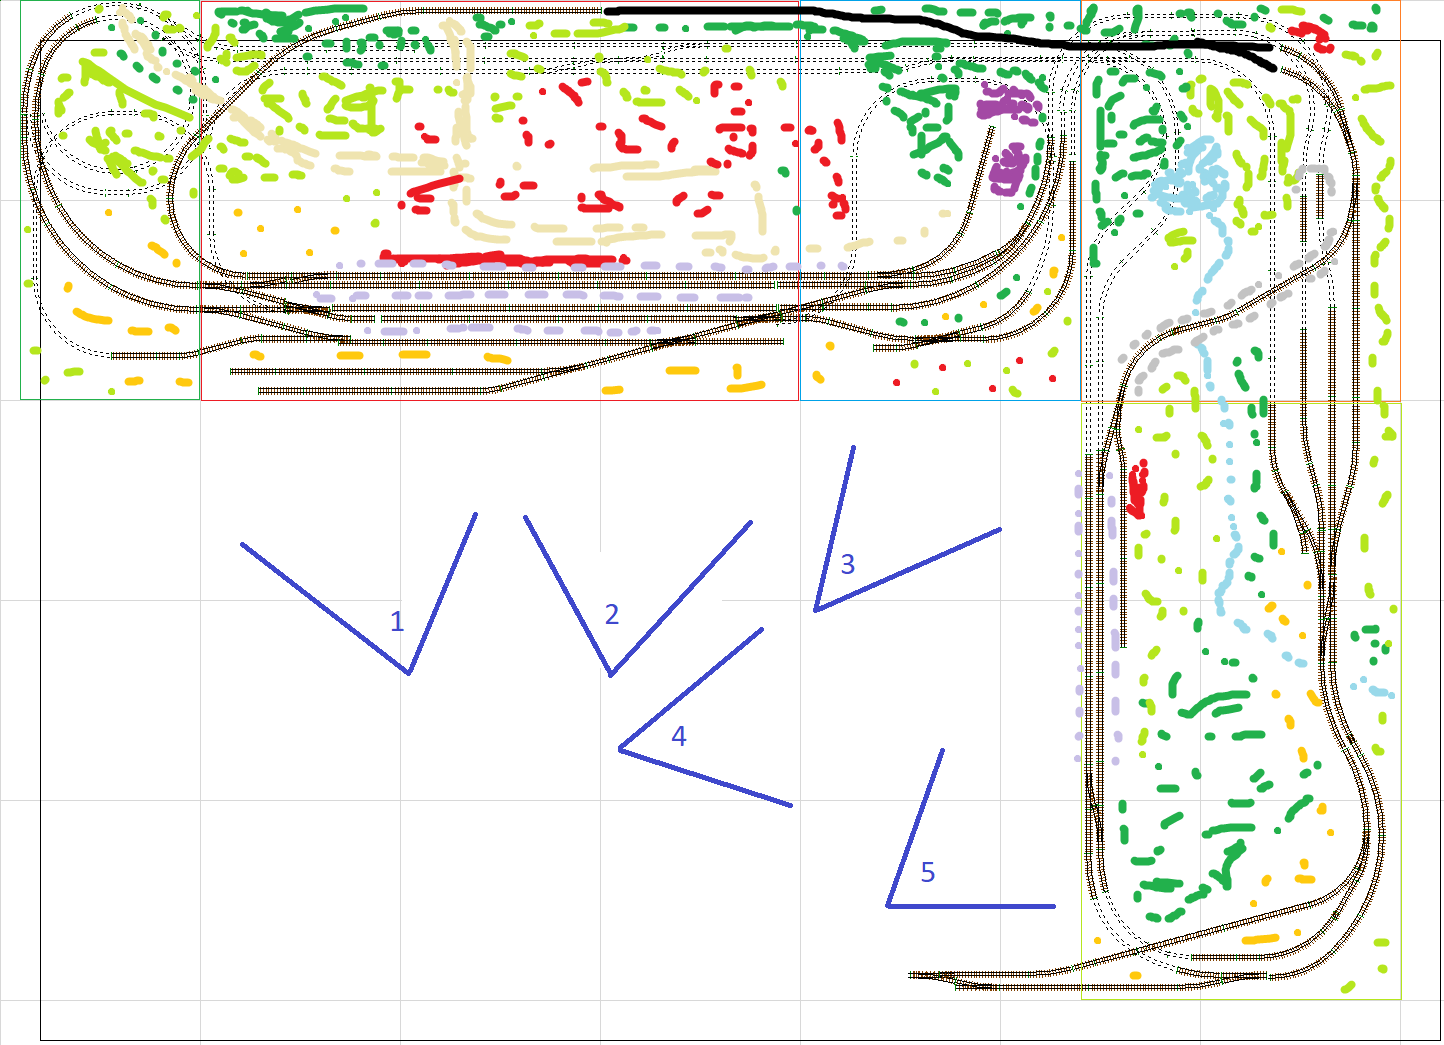
\includegraphics[width=1.0\textwidth]{img/map_evolution/state2_granitz_modules_details.png}
	\caption{Abgeknickte Acht mit flexiblerer Einbindung des Schattenbahnhofs}
	\label{img:state2_granitz_modules_details}
\end{figure}

Dieses Konzept hat tats\"achlich schon viel von der finalen Umsetzung.
De facto ist es nach wie vor ein zur Acht modifiziertes Oval.
Durch die nun aber r\"aumlich viel deutlicher abgetrennten Abzweige in die Schattenbahnhofsebene und angepassten Gleiswechsel, k\"onnen aber auch spannendere Varianten f\"ur Punkt zu Punkt Verbindungen mit dem Schattenbahnhof gefahren werden.
Die grunds\"atzliche Erweiterbarkeit an der Kehrkurve im S\"udosten w\"urde dar\"uber hinaus viel Potenzial bieten, und sei es nur durch einen weiteren Geisterbahnhof.
\begin{itemize}
	\item Der Schattenbahnhof wird ab diesem Stadium als \textbf{Schattenwalde} gelistet
	\item Der Schattenbahnhof kann zus\"atzlich auch als fiktives Alternativziel in der Ferne verwendet werden, denn \"Uberf\"uhrungsfahrten sind von Granitz aus jeweils im Osten und Westen m\"oglich sowie nach wie vor einmal an der Gleisgabelung.
\end{itemize}
Zwischenzeitlich war sogar noch eine \"Uberf\"uhrung vom Bahnhof Sch\"onblick geplant.
Diese wurde zum einen wegen des gro{\ss}en zu \"uberwindenden H\"ohenunterschieds und zum anderen im Sinne von too much verworfen.

Die Gesamtl\"ange der Anlage sowie ihre L-Form erm\"oglichen gem\"a{\ss} oben ausgef\"uhrten Punkten nun mehrere Blickwinkel des Betrachters, die auch in Fig.~\ref{img:state2_granitz_modules_details} markiert sind:
\begin{enumerate}
	\item Der Bahnhof von Granitz mit der Westausfahrt, dahinter das Alleenpanorama sowie einen Teil der Stadt
	\item Den Ostbereich des Bahnhofs von Granitz mitsamt der angrenzenden Industriebrache und nach hinten verlagerten Panoramastrecke der Nebenbahn
	\item Das fast ausschlie{\ss}lich durch den Schwenk der Nebenbahn dominierte Diorama von Sch\"onblick samt der nun vorgelagerten Wiese und Teich, seitlich begrenzt durch die R\"uckf\"uhrung der Nebenstrecke in Richtung Regiohalt
	\item Der Regiohalt Granitz-Walddorf, umgeben vom Wald mit Bachlauf
	\item Die S\"udostkehre und der Blick auf die Gleisgabel im Hintergrund
\end{enumerate}

Abschlie{\ss}end zu diesem Konzept sollen die M\"oglichkeiten betrachtet werden, die der Bahnhof Granitz selbst liefert.
Das h\"ochste Verkehrsaufkommen bietet dabei nat\"urlich die Hauptstrecke, die durch Nebengleise auch als Endpunkt f\"ur RB/RE Verbindungen fungieren kann.

Zun\"achst soll nun aber die Philosophie der Nebenstreckenplanung h\"oher aufgel\"ost werden.
Die Nebenstrecken seien grob wie folgt definiert:
\begin{enumerate}
	\item \textbf{Lokale Nebenstrecke:}\\
	Hierbei handelt es sich um die bisher schon behandelte Nebenstrecke, die \textbf{Granitz} \"uber \textbf{Sch\"onblick} mit \textbf{Granitz-Walddorf} verbindet.
	Sie ist nicht elektrifiziert.
	Im Personenverkehr ist sie f\"ur Kurzz\"uge sowie Museumsfahrten vorgesehen.
	Prinzipiell ist sie auf f\"ur den G\"uterverkehr freigegeben zum Zweck von \"Uberf\"uhrungsfahrten auf die Hauptstrecke mit Transitpunkt Gleisgabel.
	\item \textbf{Nebenstrecke Schattenwalde:}\\
	Die Strecke ist elektrifiziert und in die Ostausfahrt aus Granitz integriert.
	Es findet mit der Ausfahrt eine \"Uberf\"uhrung in die Schattenbahnhofebene statt.
	Im Personenverkehr kann sie beliebige Regionalz\"uge, im G\"uterverkehr beliebige Zuggarnituren bedienen.
	\item \textbf{Nebenstrecke westliche D\"orfer:}\\
	Es handelt sich um eine nicht elektrifizierte, tendenziell stillgelegte Nebenstrecke.
	Die Ausfahrt ist im westlichen G\"uterbahnhofsbereich von Granitz verzeichnet, hier noch als \"Uberf\"uhrung zum Schattenbahnhof.
	Letzteres Konzept wurde nachfolgend aus Gr\"unden der Komplexit\"at verworfen.
	Es bleibt alternativ die Andeutung als Gleis am linksunteren Plattenende und somit m\"oglichen Anschlusspunkt f\"ur weitere, westlich anflanschbare Segmente.
	\item \textbf{Industrienebenstrecke:}\\
	Hierbei handelt es sich um den kurzen Abzweig am Ostende des stadtseitigen Personengleises im Bahnhof von Granitz, der auf das Fabrikgel\"ander einsticht.
	Mit einer weiteren Weiche wird diese Strecke ggf. geradeaus bis an den n\"ordlichen Segmentrand verl\"angert und w\"urde dann auch eine Unterf\"uhrung der lokalen Nebenstrecke erfordern.
	Sicher ist in jedem Fall, dass zu keinem Zeitpunkt die Streckenf\"uhrung \"uber das Fabrikgel\"ande hinaus in Betrieb ist:
	Diese Nebenstrecke ist definitiv stillgelegt und \"Uberwucherung ist deutlich erkennbar.
\end{enumerate}

Die Gleise im Bahnhof von Granitz seien durchnummeriert von Norden (oben) nach S\"uden (unten):
\begin{itemize}
	\item[I] Personenverkehr
	\begin{itemize}
		\item Erster Bahnsteig, direkt am Empfangsgeb\"aude
		\item Bedienung Hauptstrecke und lokale Nebenstrecke
		\item Regul\"are Kapazit\"at: 6 Personenwagen + Lok
		\item Erweiterbare auf: 7 Personenwagen + Lok
		\item Es bleibt eine direkte Versorgung des anschlie{\ss}enden, im sp\"ateren Verlauf auf der Zeitschiene stillgelegten Fabrikgel\"andes m\"oglich.
	\end{itemize}
	\item[II] Personenverkehr und allgemeiner Durchfahrtsverkehr
	\begin{itemize}
		\item Zweiter Bahnsteig
		\item Bedienung der Hauptstrecke
		\item Kapazit\"at: 5 Personenwagen + Lok oder 6 Personenwagen mit z.T. vorgelagerter Lok
	\end{itemize}
	\item[III] Personenverkehr und allgemeiner Durchfahrtsverkehr
	\begin{itemize}
		\item Zweiter Bahnsteig, s. Gleis II
	\end{itemize}
	\item[IV] Personenverkehr
	\begin{itemize}
		\item Dritter Bahnsteig
		\item Bedienung der Hauptstrecke von Westen her mit Endpunkt Granitz
		\item Kapazit\"at: 4 Personenwagen + Lok
		\item Lokomotivumstellung \"uber Gleis V durchf\"uhrbar
	\end{itemize}
	\item[V] Personenverkehr und G\"uterverkehr (Durchfahrt, Zwischenrangierung)
	\begin{itemize}
		\item Dritter Bahnsteig
		\item Bedienung der Nebenstrecke Schattenwalde und ggf. Hauptstrecke von Osten her mit Endpunkt Granitz
		\item Kapazit\"at: 4 Personenwagen + Lok
		\item Lokomotivumstellung \"uber Gleis IV durchf\"uhrbar, alternativ in angepasstem Szenario auch \"uber Gleis VI
	\end{itemize}
	\item[VI] G\"uterverkehr
	\begin{itemize}
		\item Allgemeiner G\"uterverkehr
		\item Direkte Zufuhr von Osteinfahrt, Gleis II
		\item Abfuhr Ostausfahrt nur \"uber Verl\"angerung Gleis IV mit sp\"aterem Wechsel auf Gleis III im verdeckten Gleisbogen
		\item Zu- und Abfuhr nach Westen nur durch Rangieren \"uber Verl\"angerung Gleis IV
	\end{itemize}
	\item[VII] G\"uterverkehr, PKW-Verladung
	\begin{itemize}
		\item Prinzipiell analog zu Gleis VI
	\end{itemize}
\end{itemize}
	
Die Rationalisierung einiger \"Uberf\"uhrungen in die Schattenbahnhofsebene erfolgte prim\"ar durch erforderte Steigungen, die f\"ur den Modelleisenbahnbetrieb nicht durchf\"uhrbar sind.
F\"ur die Westausfahrt von Granitz wurde hier erstmalig der Bau einer Gleiswendel um ca. $450^{\circ}$ als notwendig erachtet.



\subsubsection{Ann\"aherung an das Eigentliche Punkt zu Punkt Konzept}
\label{sec:map_development_state3}

Eine Abwandlung des Gleisplans stellt der Stand von Fig.~\ref{img:state3_granitz_modules} dar.
Die relativ kleine, aber entscheidende Hauptma{\ss}nahme ist im nun eingezeichneten U- bzw. J-Schenkel-Segment zu sehen.
Dieses wird genutzt, um die beiden getrennten Panoramastrecken bei Granitz-Walddorf sowie der Gleisgabelung realistischer auslaufen zu lassen.
Dies erfolgt durch die Aufgabe der Kehrkurve.
Vielmehr k\"onnen beide Strecken nun mit gr\"o{\ss}eren Initialradien auf das neue S\"udsegment abgeleitet werden.

\begin{figure}[h]
\centering
  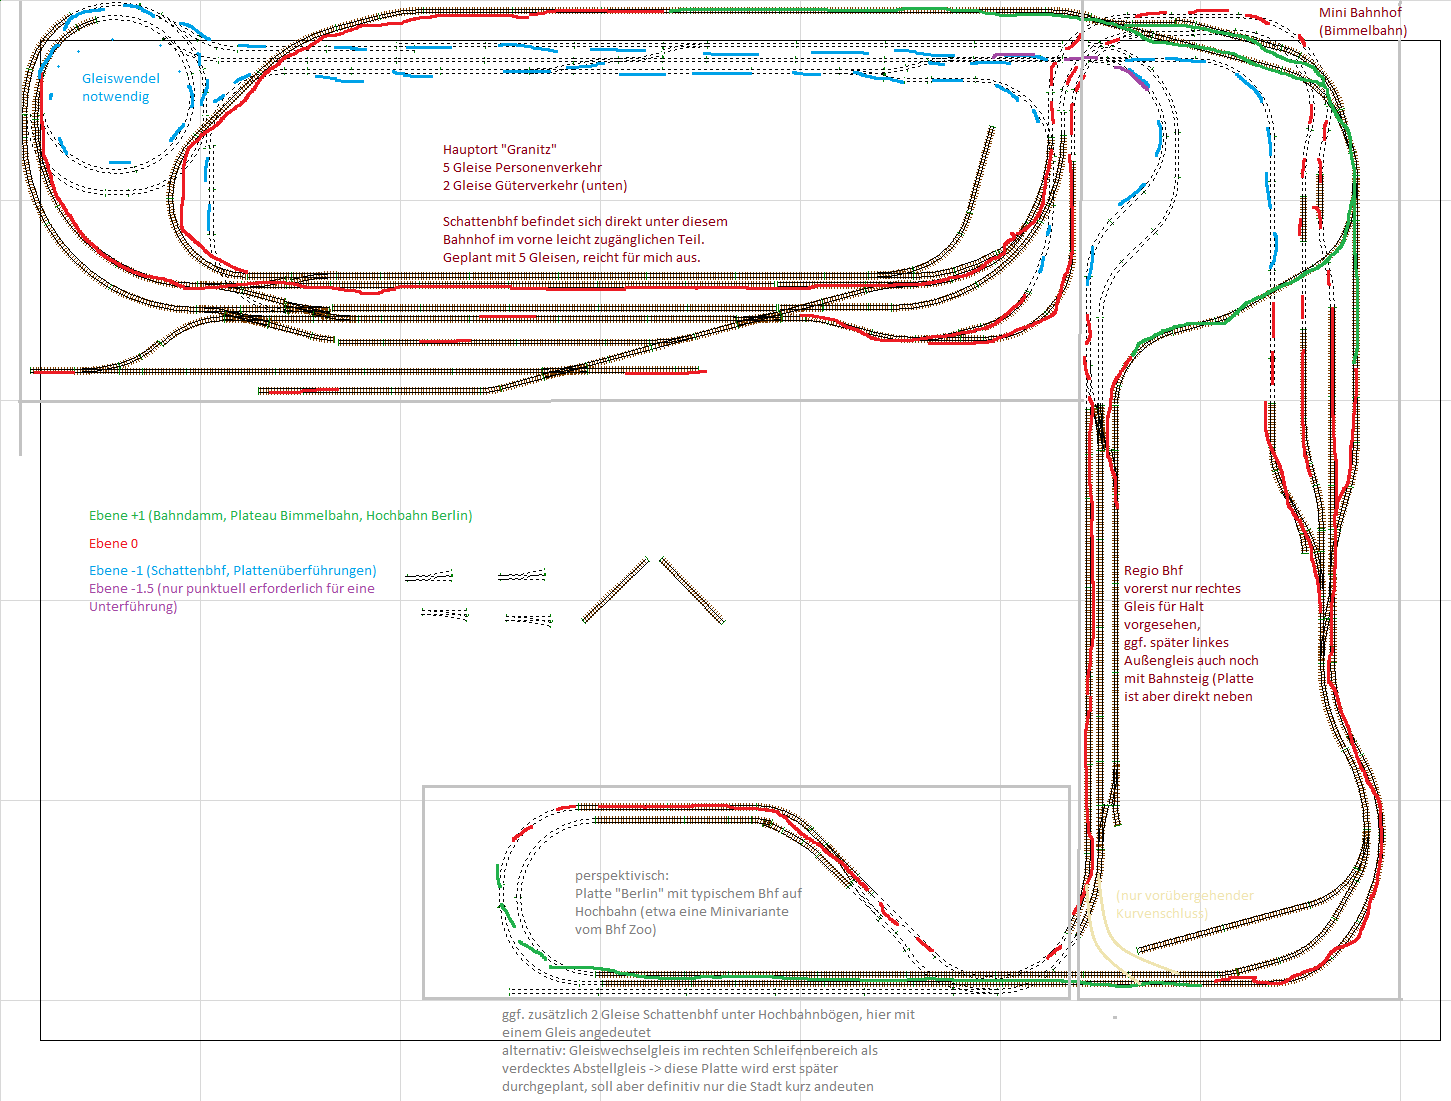
\includegraphics[width=1.0\textwidth]{img/map_evolution/state3_granitz_modules.png}
	\caption{Option zur Punkt zu Punkt Erweiterung durch Segmentierung in J-Form}
	\label{img:state3_granitz_modules}
\end{figure}

Die Ausgestaltung des S\"udsegments ist an dieser Stelle nicht entscheidend.
Verschiedene M\"oglichkeiten k\"onnen vorgesehen werden, so z.B.
\begin{itemize}
	\item wie abgebildet:
	W\"ahrend die Trasse von Granitz-Walddorf zun\"achst verdeckt gef\"uhrt wird, dann vorgelagert und in einer halben Gleiswendel m\"undet, wird die Trasse von der Gleisgabelung aus bereits auf dem Ostsegment auf eine h\"ohere Ebene verlagert und endet auf dem S\"udsegment in einem weiteren Bahnhof oder eine Panoramastrecke.
	\item operative Trennung beider Bahntrassen:
	Die Trassen erhalten verdeckt oder z.T. sichtbar Endbahnh\"ofe, so dass ein echtes Punkt zu Punkt Konzept entsteht.
	\item operative Trennung, aber mit optionaler Verbindungskehre zum Showbetrieb:
	Dieses Konzept entspricht im Prinzip dem zuvor beschriebenen, aber beh\"alt die bereits in der Abbildung angedeutete Gleiswende zumindest eingleisig bei.
	Dies erfolgt dann nur f\"ur eine noch gr\"o{\ss}ere Erweiterbarkeit der operativen M\"oglichkeiten oder der Change f\"ur einen durchgehenden Acht-Betrieb mit z.B. Kindern.
	Dieses Konzept wird nachfolgend in Sec.~\ref{sec:map_date} als aktueller Variante kurz dargestellt.
\end{itemize}
F\"ur fr\"uhe Bauphasen oder auch nur einen tempor\"aren Aufbau des S\"udsegments besteht weiterhin die M\"oglichkeit, die Kehrkurve auf dem Ostsegment durch wenige Eingriffe wiederherzustellen.
Dieser Punkt ist auch insofern wichtig, als dass mit dem Ausbau zur U-Form nun doch wieder erhebliche Zweifel am verf\"ugbaren Platz im Wohnraum aufkommen...

Ein paar kurze Worte seien noch zu sekund\"aren Modifikationen genannt:
\begin{enumerate}
	\item Die Gleise IV und VI sind \"uber die angedeutete \"Uberf\"uhrung in die stillgelegte \textbf{Nebenstrecke westliche D\"orfer} miteinander verbunden.
	Dies erm\"oglicht einen besseren Rangierbetrieb f\"ur die den St\"uckgutverkehr abwickelnden Lokomotiven.
	\item Der Bahnhof Granitz-Walddorf - zuvor f\"ur den Personenverkehr \"uber alle drei Gleise ausgelegt - ist nun auf ein bedienbares Gleis reduziert.
	Dies entspricht so manchem Vorbild von Regionalhalten in Brandenburg - gro{\ss}er Dank geht an dieser Stelle an meinen Bruder f\"ur die Idee.
	Eine Ausr\"ustung des anderen Au{\ss}engleises bleibt dennoch m\"oglicht und w\"urde das mittlere Gleis f\"ur Durchfahrten beibehalten.
	\item Ebenfalls den Bahnhof Granitz-Walddorf betreffend ist die nun beidseitige \"Uberf\"uhrungsm\"oglichkeit auf die Hauptstrecke.
	Diese wurde mit der zuvor beschriebenen Ma{\ss}nahme erforderlich.
	Zuvor endete das Gleis der \textbf{lokalen Nebenstrecke} im Bahnhof.
\end{enumerate}

Abschlie{\ss}end zeigt Fig.~\ref{img:state3_granitz_modules} eine Einf\"arbung der verschiedenen Ebenen:
\begin{itemize}
	\item Rot: Ebene 0
	\item Gr\"un: Ebene +1 (maximal $+10~cm$)
	\item Blau: Ebene -1, Schattenbahnhof (Schattenwald ca. $-15~cm$, \"Uberf\"uhrungstrasse von Granitz-West nach Granitz-Walddorf ca. $-10~cm$
	\item Gestrichelt: Allgemein verdeckter Bereich, unabh\"angig von Ebene
\end{itemize}
Es sei angemerkt, dass der Schattenbahnhof selbst wiederum nicht vollst\"andig in der Abbildung ausgef\"uhrt ist.
Allgemein befindet er sich unterhalb vom Bahnhof Granitz, einfach von der Vorderkante des Nordsegments zugreifbar.
Die hier dargestellte Version sieht den Schattenbahnhof als Kopfbahnhof vor, dessen Einfahrt unter der Westeinfahrt von Granitz Bahnhof liegt.





\subsection{Aktueller Gleisplan}
\label{sec:map_date}

Figure~\ref{img:stateDate_granitz_modules} zeigt den aktuellen Planungsstand.

\begin{figure}[h]
\centering
  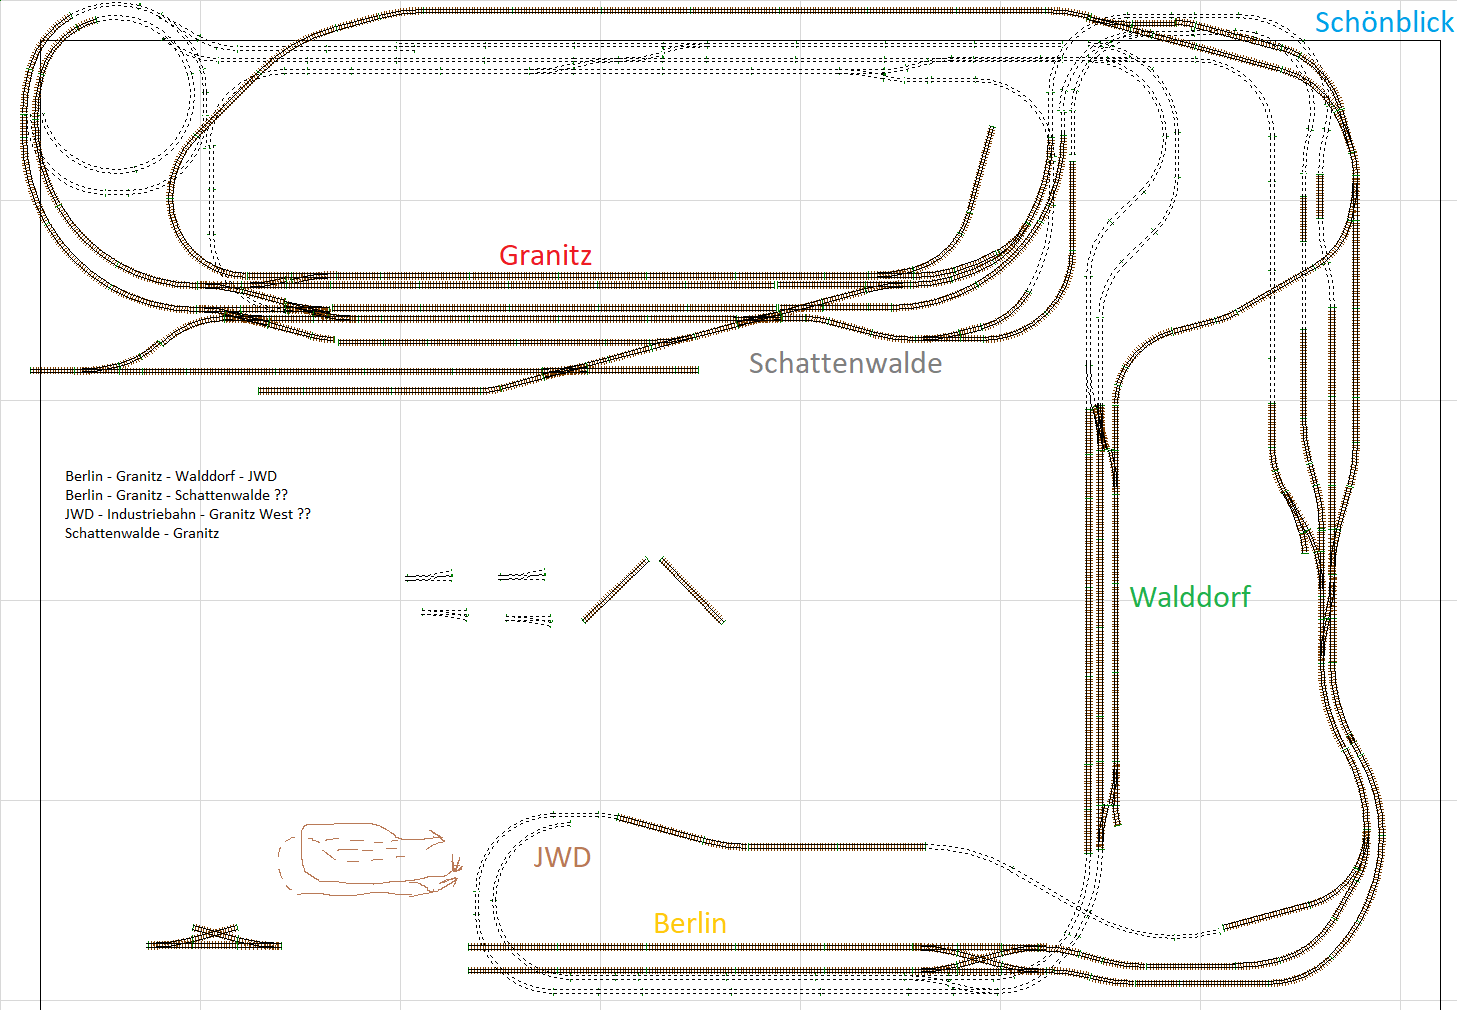
\includegraphics[width=1.0\textwidth]{img/map_evolution/stateDate_granitz_modules.png}
	\caption{Aktueller Planungsstand, auszuf\"uhren durch Segmentierung in J-Form}
	\label{img:stateDate_granitz_modules}
\end{figure}

Der wesentliche Unterschied zum Stand in Sec.~\ref{sec:map_development_state3} besteht in der bereits diskutierten Alternativausf\"uhrung vom S\"udsegment.
\begin{itemize}
	\item Endpunkt der Trasse von Granitz-Walddorf kommend ist ein kleiner Schattenbahnhof genannt \textit{JWD} (Janz weit drau{\ss}en)
	\footnote{\textit{JWD} entspringt dem Berliner und Brandenburger Jargon und bezeichnet zun\"achst alles, was weit ab vom Schuss bezeichnet.
	Von Berlin ausgesehen muss man Granitz selbst als JWD bezeichnen.
	Hier meint es aber - ausgehend von Granitz als Zentrum der Modellbahnwelt - beliebige Regional- und Fernverkehrsziele.}.
	JWD ist hier das ultimative Synonym f\"ur beliebige Ziele, die fiktiv jenseits der Modellbahnanlage sind.
	\item Endpuntk der Trasse von der Gleisgabel kommend ist ein Hochbahnhof.
	Dieser k\"onnte z.B. an den Berliner Bahnhof Zoologischer Garten angelehnt sein.
	Aus diesem Grund wird das S\"udsegment sicherlich auch in nachfolgenden immer wieder als \textbf{Berlin} bezeichnet werden.
\end{itemize}

Der ultimative Knackpunkt im f\"ur den finalen Ausbaustand anvisierten Konzept ist aber die Kehre im S\"udsegment.
Diese verbindet nun letztlich den Schattenbahnhof JWD eingleisig mit einer neuen Nebenstrecke, welche s\"udlich von der Gleisgabelung in die Hauptstrecke aufgeht.
Die szenische Ausgestaltung ist noch nicht fixiert.
Zwei Optionen werden gehandelt:
\begin{enumerate}
	\item Bahnschneise in Berlin (in dieser Form als ziemlich un\"ublich angesehen)
	\item Dioramatechnisch vom Bahnhof abgehobene Industrienebenstrecke in oder bei Berlin (der Cut in der Szenerie ist hier der Nachteil)
\end{enumerate}
Eine totale Verdeckung ist ebenfalls denkbar, w\"are aber schade.
Gerade hier bietet sich die M\"oglichkeit einer weiteren Panoramafahrt.

Allgemeinhin soll diese neue Nebenstrecke aber dem G\"uterverkehr vorbehalten sein.

F\"ur das S\"udsegment wurden insbesondere hinsichtlich der Lage des potenziellen Hochbahnhofs verschiedenste Varianten skizziert.
Da nach wie vor die Bahnsteigkapazit\"aten von mindestens, eher mehr als f\"unf Personenwagen bestehen, ist die Segmentl\"ange entsprechend zu w\"ahlen.
Kompromisse sind nicht m\"oglich, da wir hier immer noch von Berlin sprechend, das keine niedrigere Kapazit\"at als Granitz haben kann!
Zugleich offenbart sich, wie schon in Sec.~\ref{sec:map_development_state3} beschrieben, hier ein praktisches Problem:
Die Begrenzung des f\"ur die Anlage nutzbaren Raums.




\subsection{Projektierter Endausbau}
\label{sec:map_final_projected}

Eine konkrete Endausbaustufe wird hier nicht vorgestellt.
Es existieren aber folgende Grundideen:
\begin{enumerate}
	\item Ausnutzung der Minus 1 Ebenenvom Ost- und ggf. S\"udsegment f\"ur Nebenstrecken, insbesondere Dioramabildung.\\
	$\rightarrow$ nach Abschluss des aktuellen Planungsstands prinzipiell jeder Zeit zumindest f\"ur das Ostsegment realisierbar
	\item Erweiterung des Rangierbereichs vom G\"uterbahnhof Granitz durch Anschluss eines Segments an Granitz-West.
	Dieser w\"urde dann den nicht mehr bewirtschafteten \"Ubergang zur \textbf{Nebenstrecke westliche D\"orfer} andeuten.\\
	$\rightarrow$ als weites Fernziel realisierbar, da hier aktuell ein selbstgebautes, gro{\ss}fl\"achiges Regal anschlie{\ss}t, von dem entsprechend ein Fach ger\"aumt werden m\"usste
	\item Reaktivierung der \textbf{Nebenstrecke westliche D\"orfer} durch Anschluss eines Segments an Granitz-West.
	Analog zu vorherigem Konzept, aber mit weniger Rangierfl\"ache, daf\"ur einer weiteren Gleiswendel, welche letztendlich Erweiterungen in einer weit \"uber Granitz gelagerten Ebene (Minimum: $70~cm$) erm\"oglichen w\"urde.\\
	$\rightarrow$ unrealistisch
	\item Nutzung des S\"udsegments f\"ur eine Gleiswendel analog zu vorherigem Konzept.
	Diese Wendel w\"urde ebenfalls eine nun neue Nebenstrecke auf einer deutlich \"uber dem Ostsegment gelagerten Ebene erlauben.\\
	$\rightarrow$ unrealistisch, da bereits das S\"udsegment mit gro{\ss}er Sicherheit nicht dauerhaft platziert werden kann
	\item Alternative Ausf\"uhrung der \textbf{Nebenstrecke westliche D\"orfer} \"uber einen nahezu O-Schluss der Segmente.
	Dies erm\"oglicht auch noch verh\"altnism\"a{\ss}ig viel L\"ange f\"ur diese Nebenstrecke.\\
	$\rightarrow$ unrealistisch, da noch mehr Platzbedarf von N\"oten und daher wenn \"uberhaupt nur in sauberer Modulbauweise umsetzbar
\end{enumerate}

%\begin{figure}[h]
%\centering
	%\begin{subfigure}[b]{0.49\textwidth}
    %\includegraphics[width=1.0\textwidth]{sub/concept_studies/img/carpets/benefit_maps/map_benefit_s500.png}
   %\caption{$s = 500 NM$}
    %\label{img:carpets_benefit_maps_s500}
    %\end{subfigure}
	%\begin{subfigure}[b]{0.49\textwidth}
    %\includegraphics[width=1.0\textwidth]{sub/concept_studies/img/carpets/benefit_maps/map_benefit_s1000.png}
   %\caption{$s = 1000 NM$}
    %\label{img:carpets_benefit_maps_s1000}
    %\end{subfigure}
		%\begin{subfigure}[b]{0.49\textwidth}
    %\includegraphics[width=1.0\textwidth]{sub/concept_studies/img/carpets/benefit_maps/map_benefit_s2500.png}
   %\caption{$s = 2500 NM$}
    %\label{img:carpets_benefit_maps_s2500}
    %\end{subfigure}
		%\begin{subfigure}[b]{0.49\textwidth}
    %\includegraphics[width=1.0\textwidth]{sub/concept_studies/img/carpets/benefit_maps/map_benefit_s5000.png}
   %\caption{$s = 5000 NM$}
    %\label{img:carpets_benefit_maps_s5000}
    %\end{subfigure}
	%\caption{Straight map of benefits for PSN supply flow modulation}
	%\label{img:carpets_benefit_maps}
%\end{figure}